\section{Sp\-String.h File Reference}
\label{SpString_8h}\index{SpString.h@{SpString.h}}
{\tt \#include $<$string$>$}\par
{\tt \#include $<$sstream$>$}\par
{\tt \#include $<$vector$>$}\par
{\tt \#include $<$list$>$}\par
{\tt \#include \char`\"{}Sp\-String.inc\char`\"{}}\par


Include dependency graph for Sp\-String.h:\begin{figure}[H]
\begin{center}
\leavevmode
\includegraphics[width=171pt]{SpString_8h__incl}
\end{center}
\end{figure}


This graph shows which files directly or indirectly include this file:\begin{figure}[H]
\begin{center}
\leavevmode
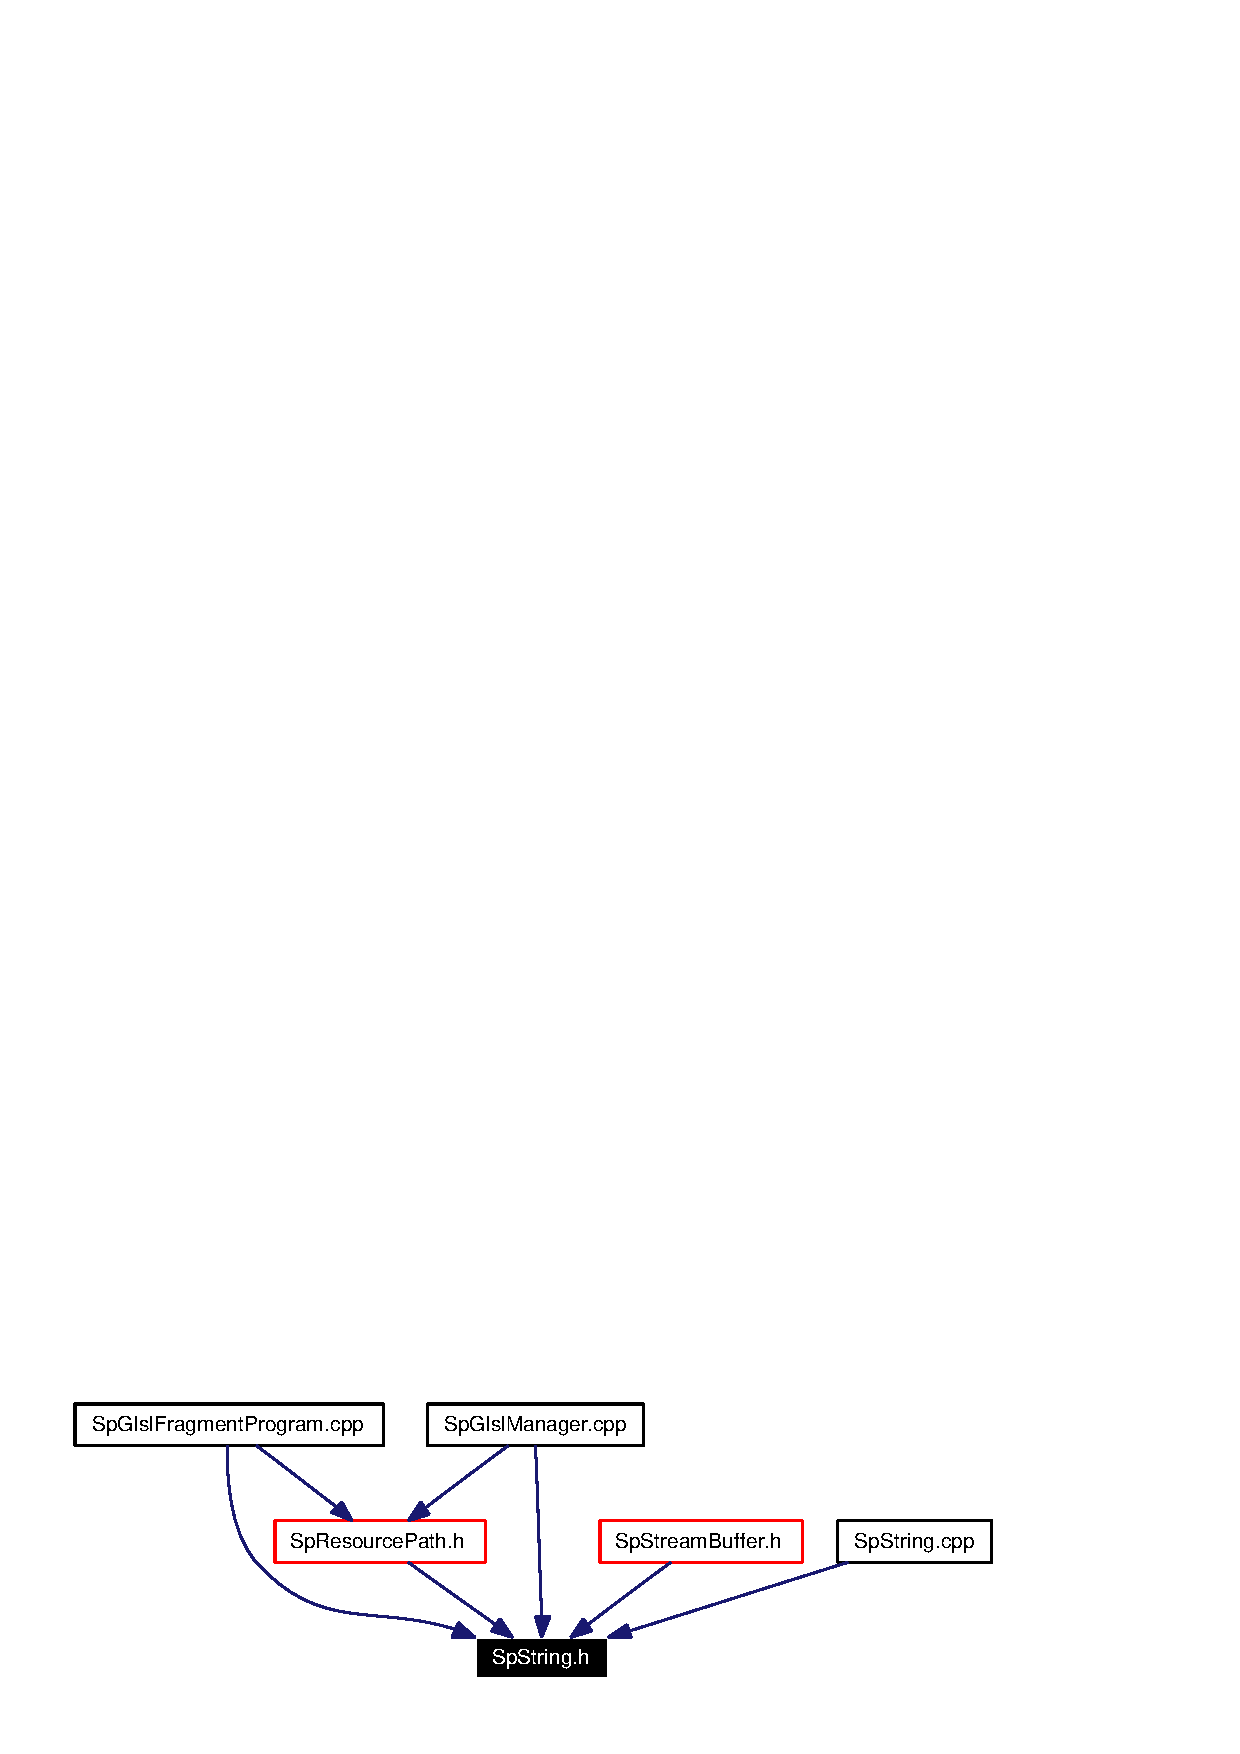
\includegraphics[width=238pt]{SpString_8h__dep__incl}
\end{center}
\end{figure}
\subsection*{Namespaces}
\begin{CompactItemize}
\item 
namespace {\bf Spark}
\end{CompactItemize}
\subsection*{Classes}
\begin{CompactItemize}
\item 
class {\bf Spark::Sp\-String}
\begin{CompactList}\small\item\em String utility class for character data. \item\end{CompactList}\end{CompactItemize}
\subsection*{Typedefs}
\begin{CompactItemize}
\item 
typedef std::string {\bf Sp\-String\-Base}
\item 
typedef std::stringstream {\bf Sp\-String\-Stream\-Type}
\item 
typedef std::vector$<$ {\bf Sp\-String} $>$ {\bf Sp\-String\-Array}
\item 
typedef std::list$<$ {\bf Sp\-String} $>$ {\bf Sp\-String\-List}
\item 
typedef std::pair$<$ {\bf Sp\-String}, {\bf Sp\-String} $>$ {\bf Sp\-String\-Pair}
\end{CompactItemize}


\subsection{Typedef Documentation}
\index{SpString.h@{Sp\-String.h}!SpStringArray@{SpStringArray}}
\index{SpStringArray@{SpStringArray}!SpString.h@{Sp\-String.h}}
\subsubsection{\setlength{\rightskip}{0pt plus 5cm}typedef std::vector$<${\bf Sp\-String}$>$ {\bf Spark::Sp\-String\-Array}}\label{namespaceSpark_a4}


Definition at line 49 of file Sp\-String.h.

Referenced by Spark::Sp\-Resource\-Path::searchpath().\index{SpString.h@{Sp\-String.h}!SpStringBase@{SpStringBase}}
\index{SpStringBase@{SpStringBase}!SpString.h@{Sp\-String.h}}
\subsubsection{\setlength{\rightskip}{0pt plus 5cm}typedef std::string {\bf Spark::Sp\-String\-Base}}\label{namespaceSpark_a2}


Definition at line 44 of file Sp\-String.h.

Referenced by Spark::Sp\-String::Sp\-String().\index{SpString.h@{Sp\-String.h}!SpStringList@{SpStringList}}
\index{SpStringList@{SpStringList}!SpString.h@{Sp\-String.h}}
\subsubsection{\setlength{\rightskip}{0pt plus 5cm}typedef std::list$<${\bf Sp\-String}$>$ {\bf Spark::Sp\-String\-List}}\label{namespaceSpark_a5}


Definition at line 50 of file Sp\-String.h.\index{SpString.h@{Sp\-String.h}!SpStringPair@{SpStringPair}}
\index{SpStringPair@{SpStringPair}!SpString.h@{Sp\-String.h}}
\subsubsection{\setlength{\rightskip}{0pt plus 5cm}typedef std::pair$<${\bf Sp\-String}, {\bf Sp\-String}$>$ {\bf Spark::Sp\-String\-Pair}}\label{namespaceSpark_a6}


Definition at line 51 of file Sp\-String.h.\index{SpString.h@{Sp\-String.h}!SpStringStreamType@{SpStringStreamType}}
\index{SpStringStreamType@{SpStringStreamType}!SpString.h@{Sp\-String.h}}
\subsubsection{\setlength{\rightskip}{0pt plus 5cm}typedef std::stringstream {\bf Spark::Sp\-String\-Stream\-Type}}\label{namespaceSpark_a3}


Definition at line 48 of file Sp\-String.h.